\documentclass[a4paper,12pt]{article}
\usepackage{graphicx}
\usepackage[ngerman]{babel}
\usepackage[ansinew]{inputenc}
\usepackage{amsmath}
\usepackage{amsfonts}
\usepackage{graphicx}

\usepackage{scrpage2}
\cfoot{Realgymnasium Albert Einstein - Meran}
\setheadsepline{.04pt}
\setfootsepline{.04pt}
\pagestyle{scrheadings}
\ohead{}
\ihead{\headmark}


\begin{document}
\begin{center}
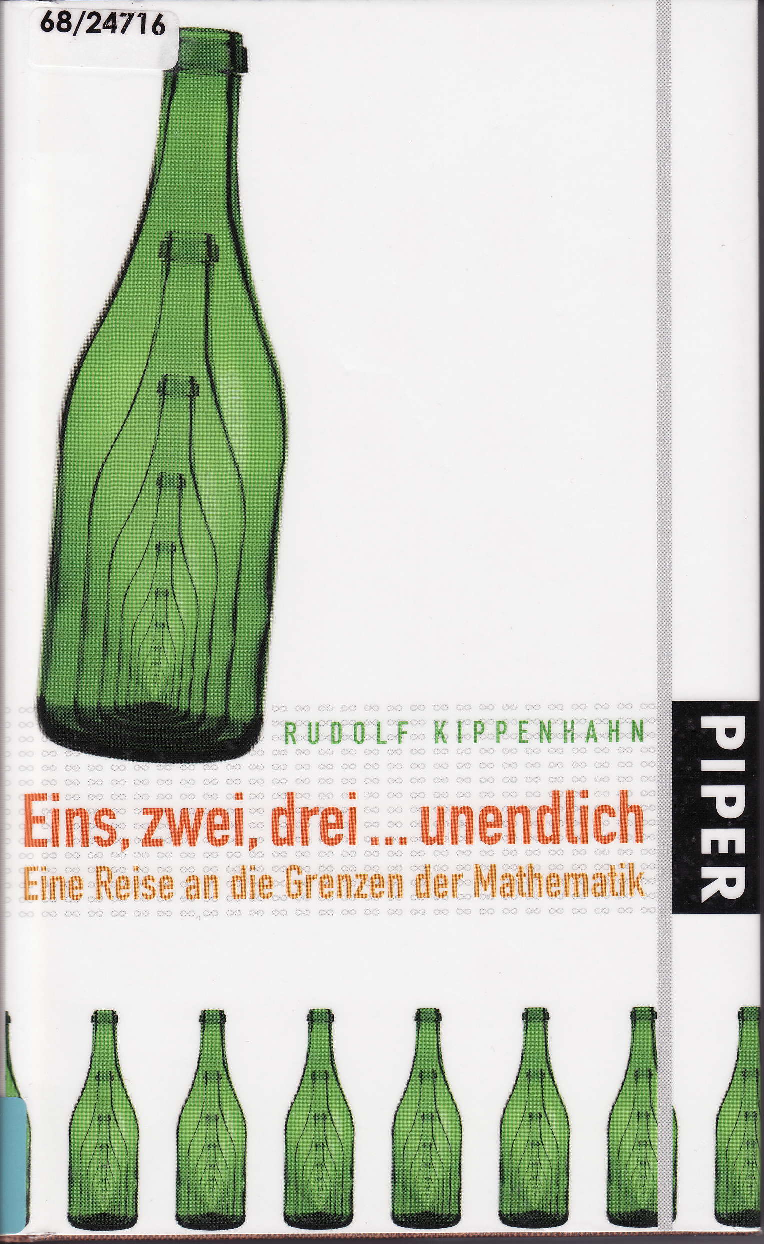
\includegraphics[width=12 cm]{IMG.pdf}
\end{center}

\newpage

\begin{center}
 \large{\textbf{Eins, zwei, drei...unendlich}}\newline 
\end{center}
\begin{center}
\large{\textit{Eine Reise bis an die Grenzen der Mathematik}}\newline
\end{center}

\begin{center}
\large{von Rudolf Kippenhahn}\newline
\end{center}
\newline

\begin{center}
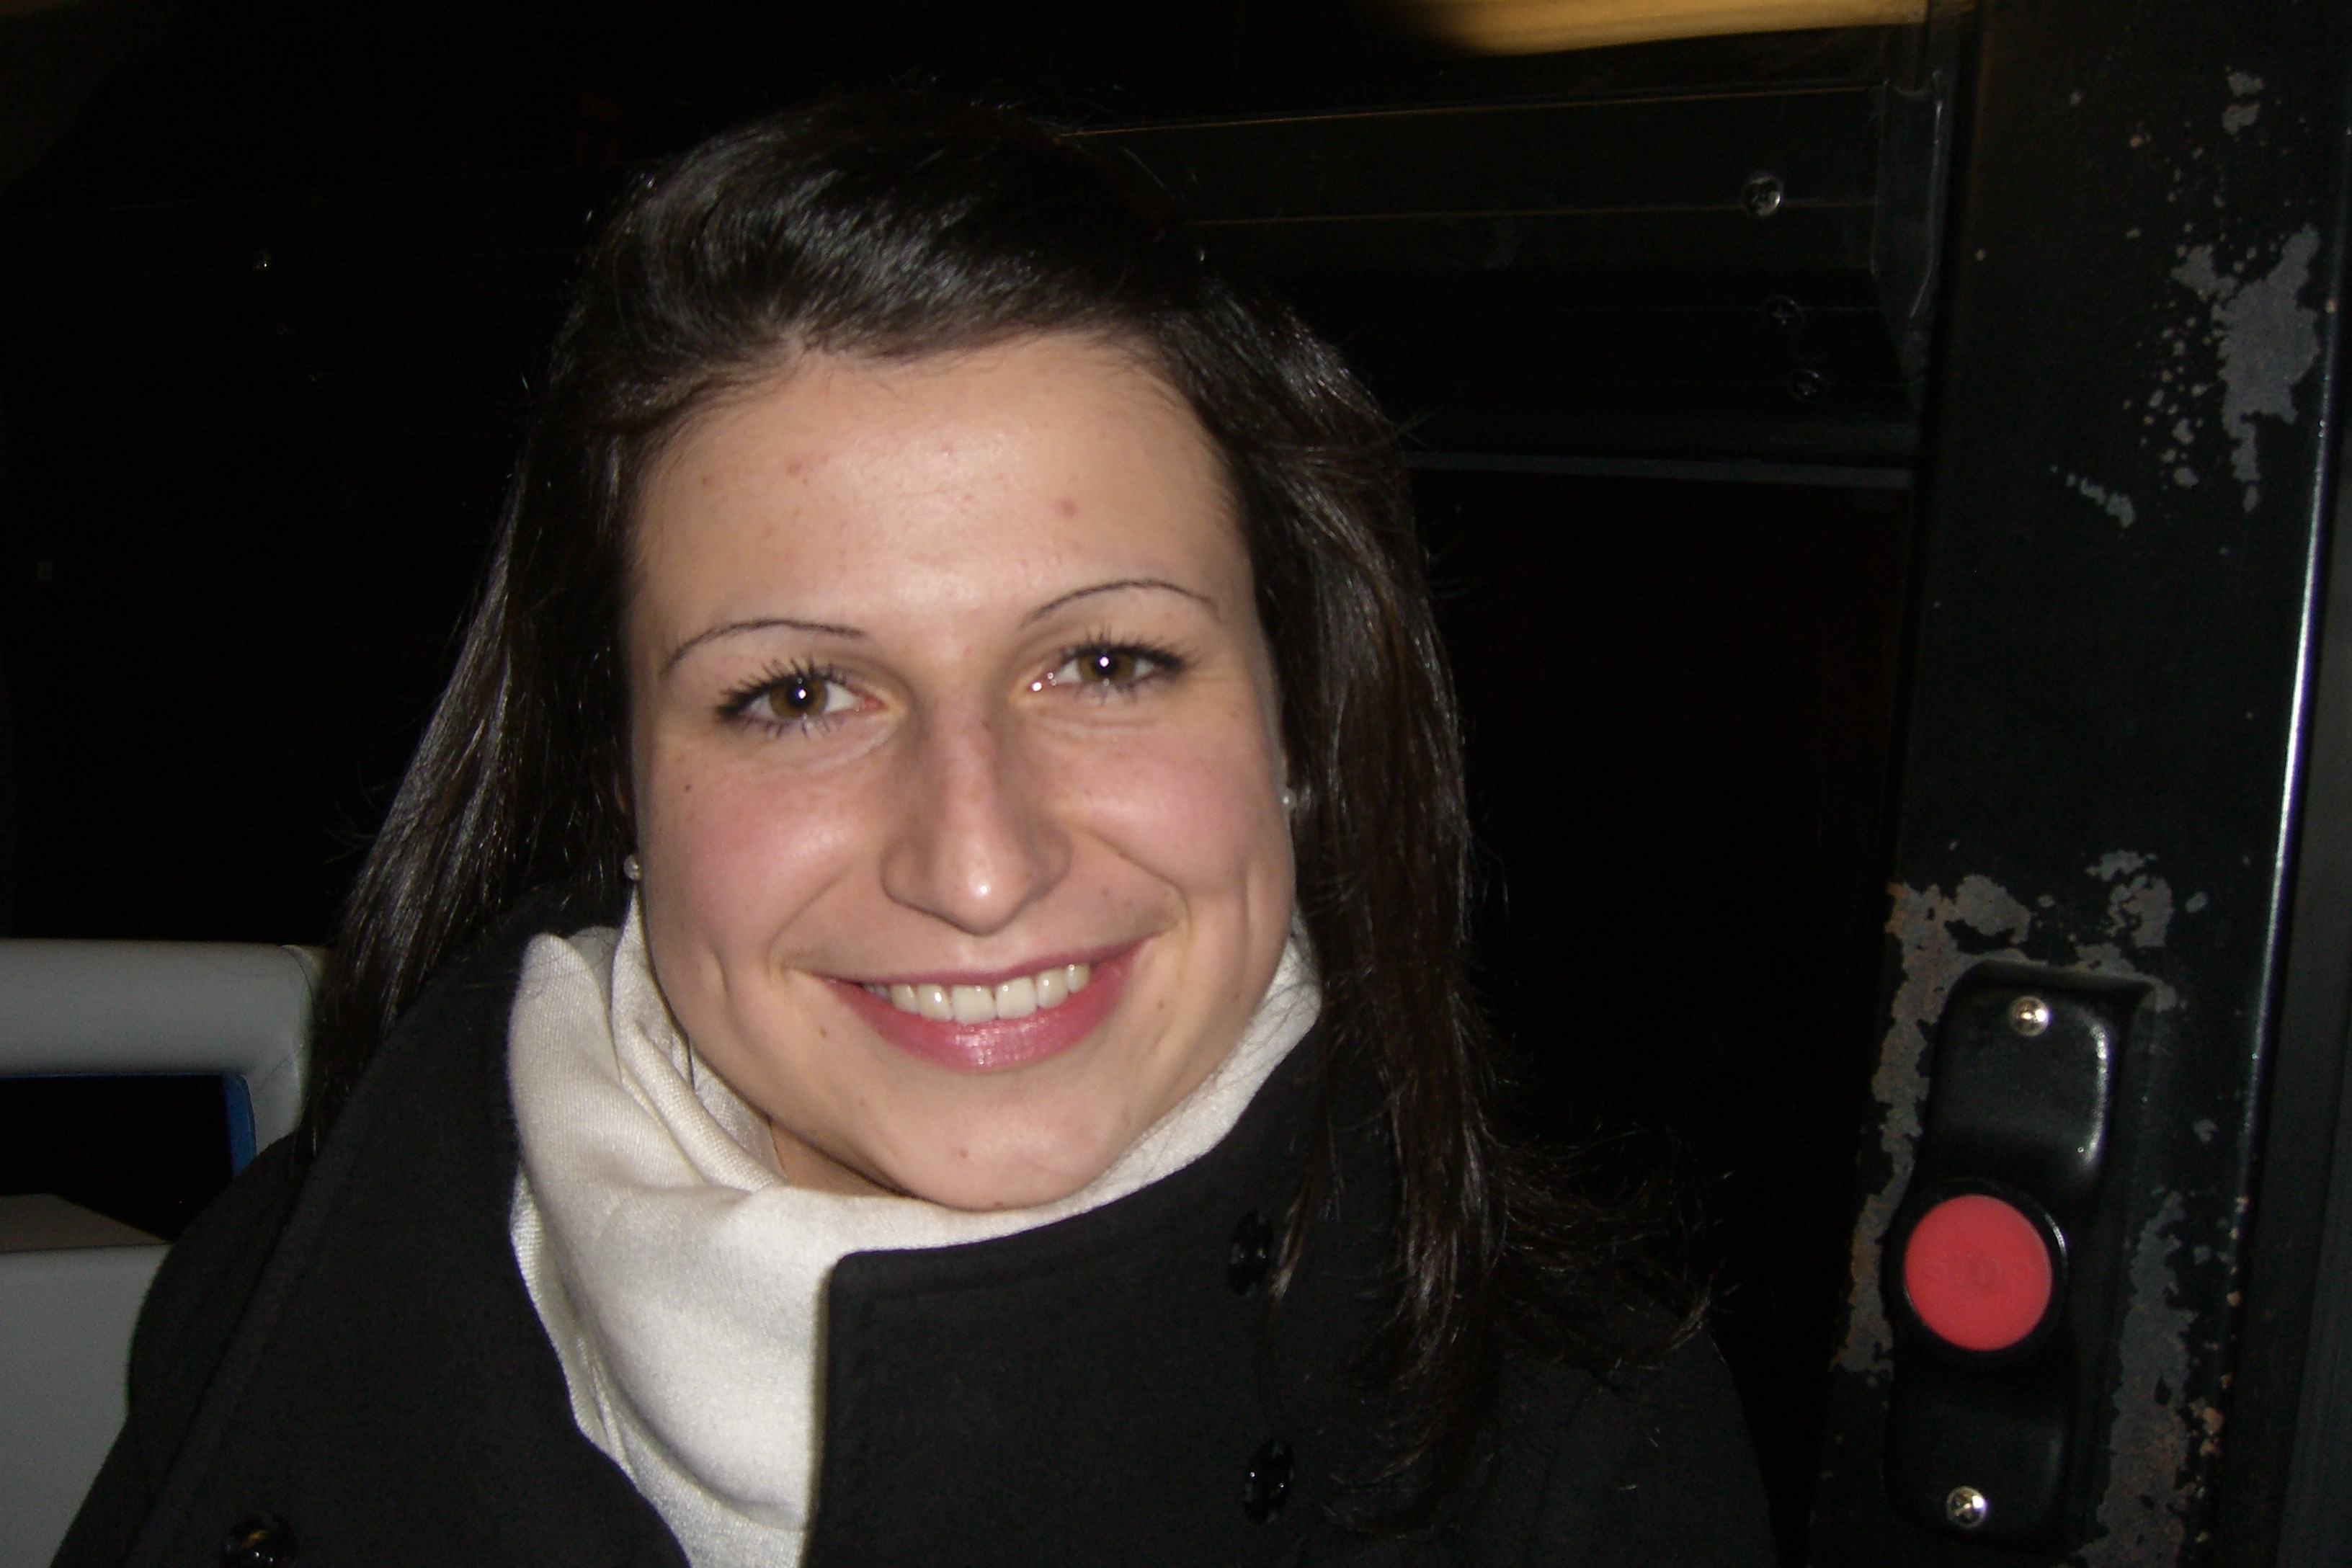
\includegraphics[width=4 cm]{portrait.jpg}
\end{center}

\begin{center}
 \large{Eine Buchbesprechung von Christa Ungericht}
\end{center}
\newpage

\section{Der Autor}\newline
\begin{center}	
		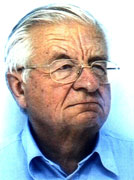
\includegraphics[width=3 cm]{RKip.jpg}
\end{center}

Rudolf Kippenhahn wurde 1926 in Bärringen (Böhmen) geboren und ist Mathematiker und Astrophysiker. Bereits als Schüler arbeitete er in einer Sternwarte und studierte später Mathematik. Er entdeckte seine Leidenschaft für Astronomie und Astrophysik und lehrte diese Fächer von 1965 bis 1975 an der Universität in Göttingen. Daraufhin war er bis 1991 Direktor des Max- Planck- Institutes für Astrophysik in Garching bei München. In diesem Jahr wurde zudem der kleine Planet 2947 nach seinem Nachnamen benannt. Seit einigen Jahren lebt Rudolf Kippenhahn als Schriftsteller in Göttingen; er schreibt regelmäßig Kolumnen für astronomische Zeitschriften. Außerdem hat Kippenhahn bisher 16 erfolgreiche Sachbücher veröffentlicht, darunter zwei Kinderbücher.

\section{Zum Inhalt des Buches}\newline
Rudolf Kippenhahn vermittelt auf eine für Laien verständliche Weise einen Einblick in das Reich des Unendlichen. Einfache mathematische Erläuterungen sorgen dabei für einwandfreie Verständlichkeit bei der Behandlung verschiedener Themenbereiche.
Der Inhalt kommt durch die verwendete Schreibform, den Dialog, besonders gut rüber. Im Text nimmt der junge Alex die Position des Lesers ein; aufkommende Fragen zum Inhalt werden von ihm an seinen Großvater, den Erzähler, gestellt.
Das Buch verknüpft alltägliche Situationen und Geschehnisse mit dem umstrittenen Thema der Unendlichkeit. So werden beispielsweise folgende Fragen behandelt:\newline
Gibt es gleich viele gerade Zahlen wie ungerade? Gibt es mehr Brüche als Zahlen? Ist der Weltraum wirklich unbegrenzt? Wie steht die Unendlichkeit in Zusammenhang mit Mathematik, Physik und Astronomie?\newline
Gleich zu Beginn des Buches wird die Geschichte der rätselhaften Flasche behandelt: Man stelle sich eine Flasche vor, sagen wir eine Ketchupflasche, auf deren Etikett ein Zwerg abgebildet ist, der wiederum auf eine Flasche schaut. Auch diese Flasche hat dasselbe Etikett, nur kleiner: einen Zwerg, der auf eine Flasche schaut. Und so geht es immer weiter, bis in die Unendlichkeit. Natürlich lassen sich schon bald keine Einzelheiten mehr erkennen, da die Etiketten sehr klein werden, aber rein gedanklich kann man sich dies vorstellen.
Eine weitere nette Spielerei mit der Unendlichkeit ist das \textit{Hilberts Hotel}, ein Hotel mit unendlich vielen Zimmern. Hier stelle man sich vor, dass sich in dem Hotel unendlich viele Gäste befinden würden. Wenn nun spätabends noch ein Gast ein Zimmer buchen möchte, so schickt der Portier den Gast mit der Zimmernummer 1 ins Zimmer 2, den Gast aus Zimmer 2 ins Zimmer 3, usw.. Jeder Gast zieht in das Zimmer mit der nächsten Nummer und der Neuankömmling kann das Zimmer 1 beziehen. Die Moral von der Geschichte um \textit{Hilberts Hotel} ist diese:\newline
\newline
unendlich + 1 = unendlich\newline
\newline
Solche und noch weitere nette Geschichten rund um die Unendlichkeit werden in diesem Buch jugendgerecht und mit vielen Illustrationen behandelt.
Im Anhang sind für interessierte Leser die mathematischen Inhalte nochmals genauer ausgeführt und aufgelistet. \newline
\section{Porträt einer Hauptfigur}\newline
Das Buch handelt von einem Dialog zwischen dem Jungen Alex und seinem Großvater und ist in der ersten Person aus Sicht des Großvaters geschrieben.\newline
Alex verkörpert einen typischen Schüler: Interessiert und konzentriert, aber auch mürrisch und trotzig, wenn etwas nicht auf Anhieb so klappt wie er es möchte. Er dürfte um die 14 Jahre alt sein (dies wird im Buch nicht genau genannt).\newline
Er ist als eine der Hauptpersonen sehr gut gewählt, da er mit der Rolle des Lesers gleichgestellt wird und tiefergreifendere und deutlichere Erklärungen fordert, die auch dem Leser hin und wieder auf der Zunge brennen. Diese schwierige Aufgabe, den Dialog lehrreich und fesselnd zugleich zu gestalten hat der Autor sehr gut bewältigt.
\glqq Ich glaube, das Unendliche in meinem Kopf ist jetzt ganz anders als das Unendliche in meinem Bauch.\grqq \newline
\newline
Dies sagt Alex ganz am Ende des Buches und diese Aussage gefällt mir deshalb so gut, weil es genau meine persönlichen Gefühle nach dem Lesen dieses Buches wiederspiegelt. Die Gefühle aus dem Bauch stehen in enger Beziehung mit den täglichen Erfahrungen und lassen sich deshalb nicht genau mit der trockenen Theorie des Unendlichen verbinden. Beim Lesen des Buches wird man konsequent mit der Unendlichkeit konfrontiert und obwohl ich die Theorie verstanden habe, \textit{spüre} ich trotzdem, dass irgendetwas faul an der ganzen Sache ist. Ein gutes Beispiel hierfür ist das Weltall; wissenschaftliche Erkenntnisse zeigen, dass das Weltall unendlich ist und dennoch kann ich mir nicht wirklich vorstellen, wie es in Wirklichkeit aussieht, wie diese Unendlichkeit möglich sein soll.
\section{Meine Meinung zum Buch}\newline
Mir hat das Buch \glqq Eins, zwei, drei...unendlich\grqq\  wirklich sehr gut gefallen, weil ich vorher nicht wusste das dieser Begriff der Unendlichkeit so vielfältig und interessant ist. Wenn ich vorher \glqq unendlich\grqq\  gesagt habe, habe ich eigentlich nie darüber nachgedacht, was \glqq unendlich\grqq\  im engeren Sinn bedeutet; ich habe mit unendlich um mich geworfen, ohne nachzudenken, was alles in diesem Begriff steckt.\newline
Ich würde das Buch auf jeden Fall weiterempfehlen, da es auf einfache und verständliche Weise in die Welt der Unendlichkeit und zugleich in die Mathematik und Astronomie entführt.
\end{document}